\chapter{Analysis of Extended Cycle Shrinking Algorithm}

A dependence distance $\Phi(R)$ is called a dominating dependence distance if $\Phi(L) = \Phi(R)$. A dominating dependence distance may not always exist.  \\

The extended cycle shrinking algorithm is optimal only when there exists a dominating dependence distance. If cycle shrinking is applied to loops where this is not the case then it gives suboptimal partitions. \\

\noindent For example consider the following code: \\
DO I = 0, 9 \\
\indent DO J = 0, 9 \\
\indent \indent A[I+1, J+9] = B[I, J] \\
\indent \indent C[I+6, J+6] = A[I, J] \\
\indent \indent B[I+8, J+1] = C[I, J] \\
\indent ENDO \\
ENDO \\

The dependence distances are (1, 9), (6, 6) and (8, 1). $\Phi(L) = (1, 1)$. Thus, there is no dominating dependence distance in this case. The partitions created by extended cycle shrinking algorithm and a better possible partition is shown in Figure~\ref{fig:eg_opt}. This motivates us to optimize the extended cycle shrinking algorithm so to have optimal partitions even in those cases where there is no dominating dependence distance.\\

\begin{figure}
\centering
\begin{subfigure}{0.5\textwidth}
  \centering
  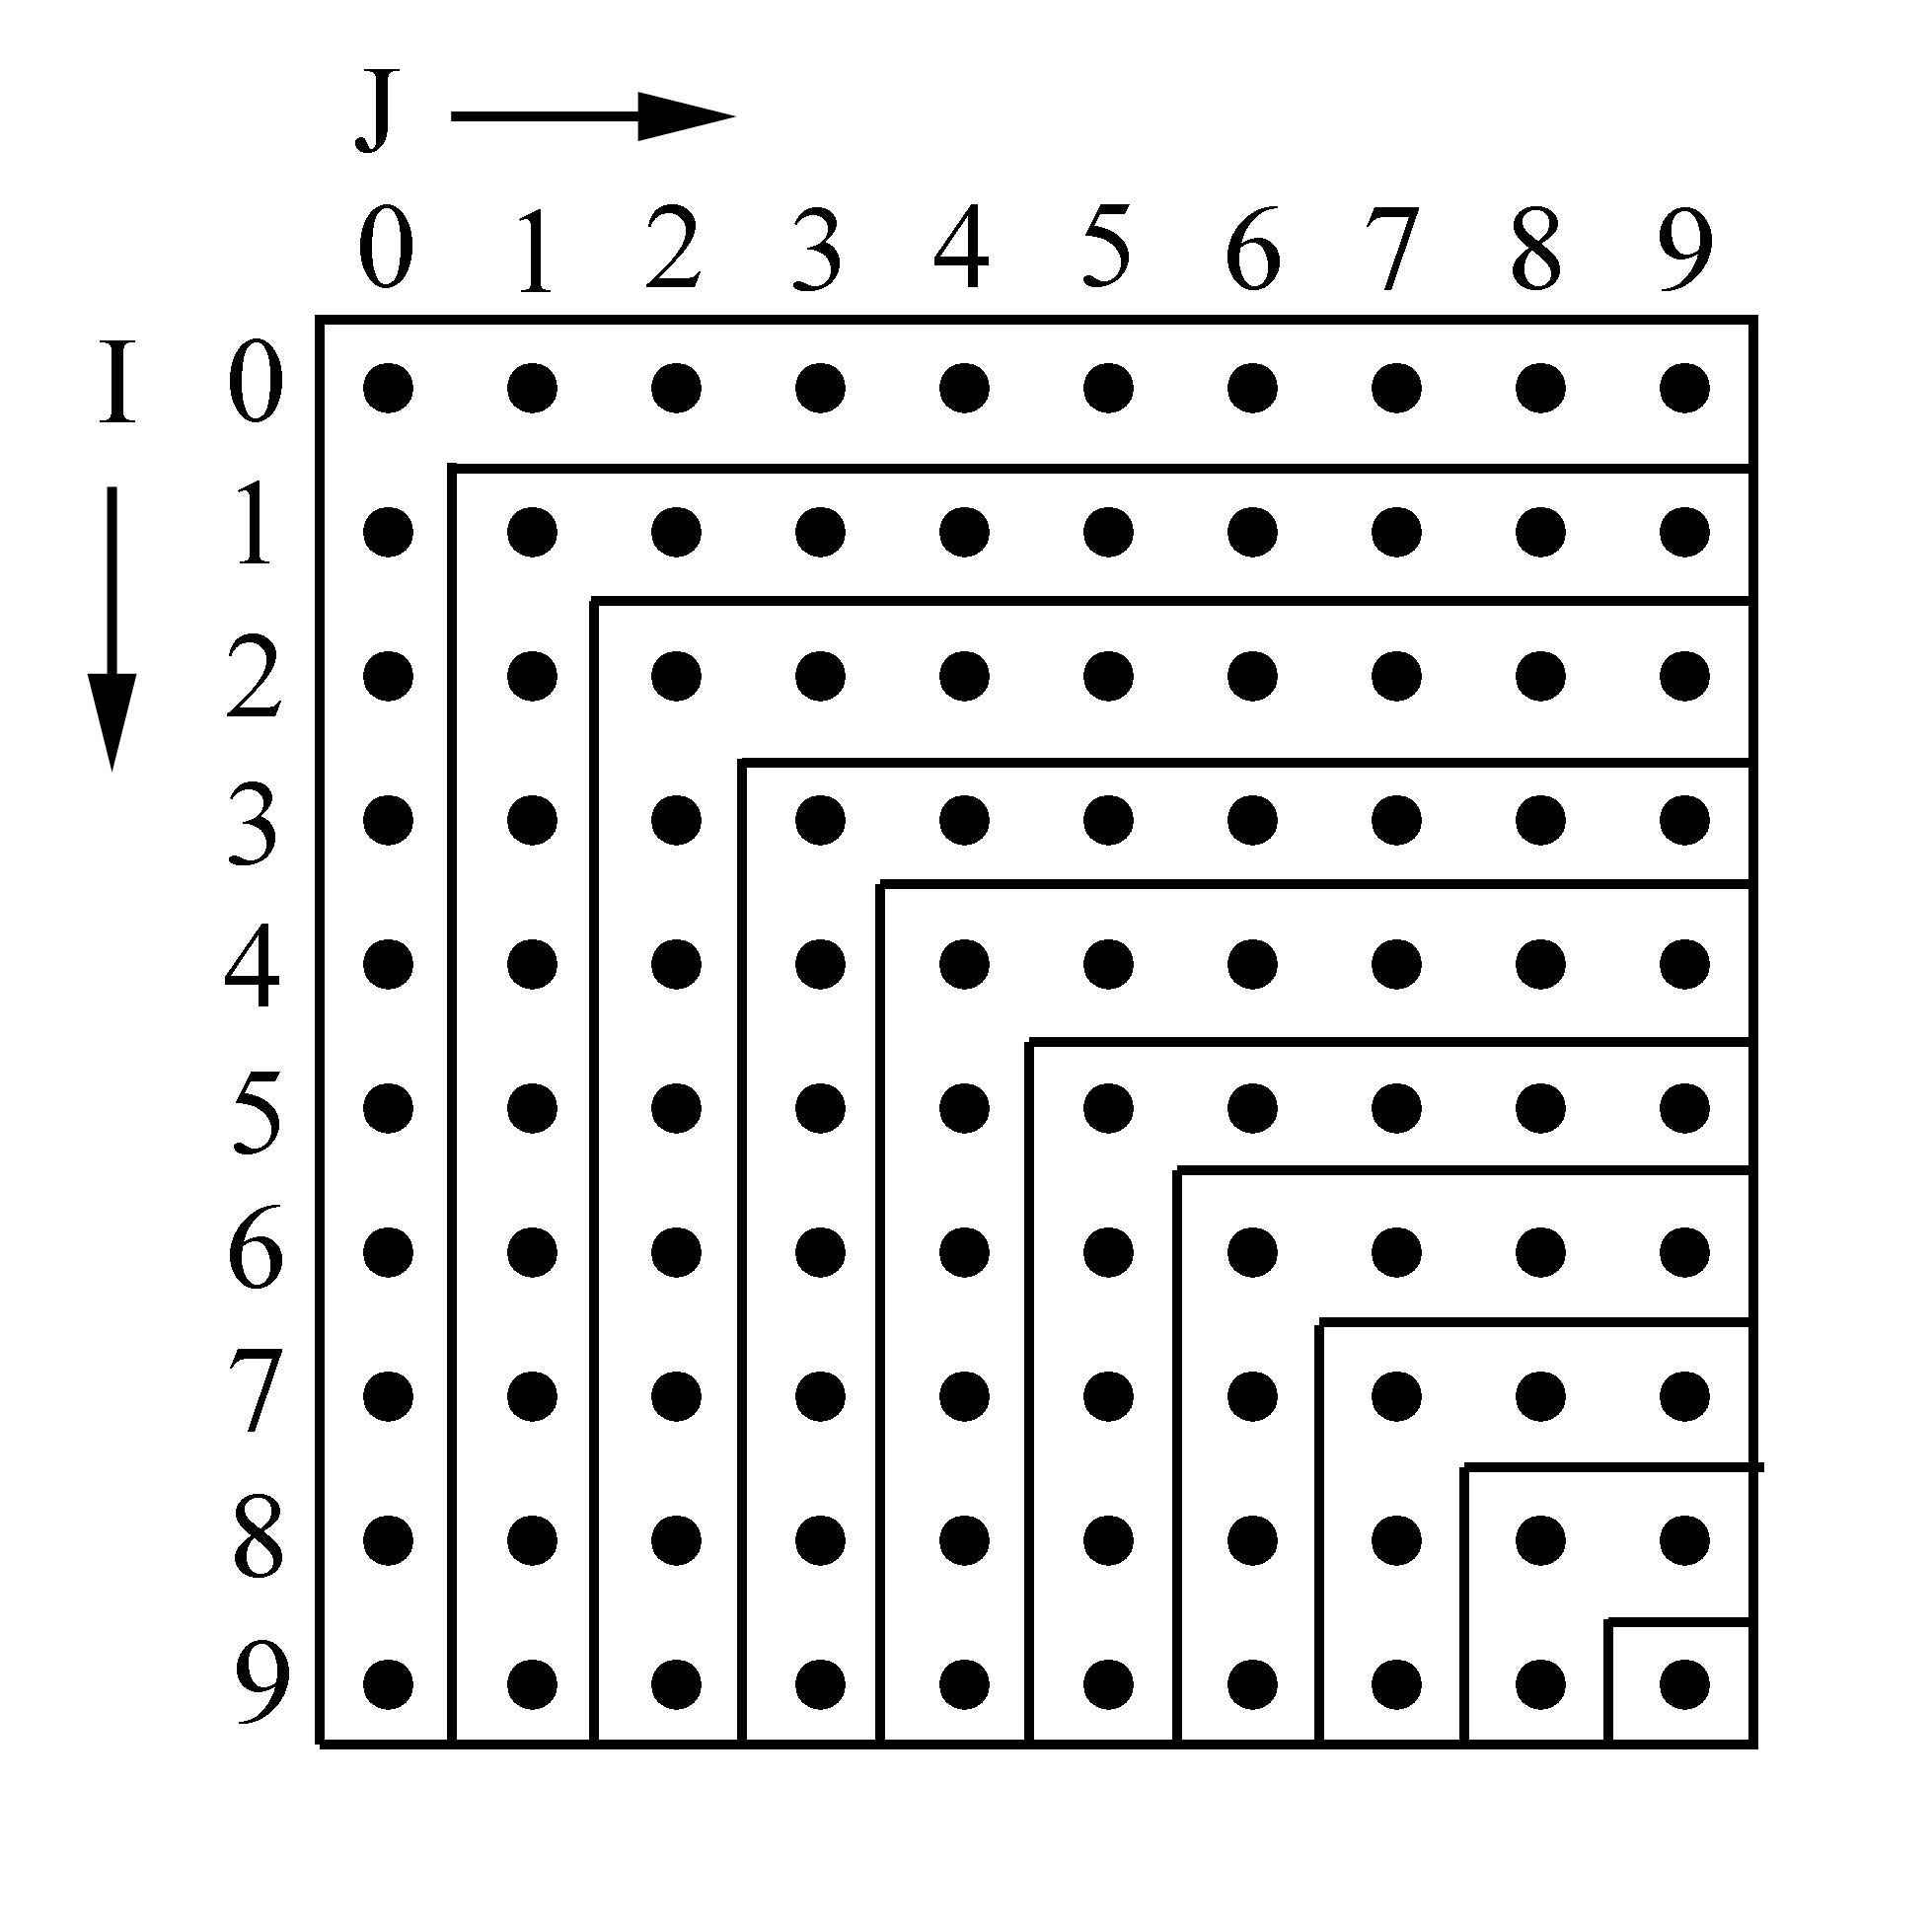
\includegraphics[width=\textwidth]{Figures/fig1a.jpg}
  \caption{}
  \label{fig:sub1}
\end{subfigure}%
\begin{subfigure}{0.5\textwidth}
  \centering
  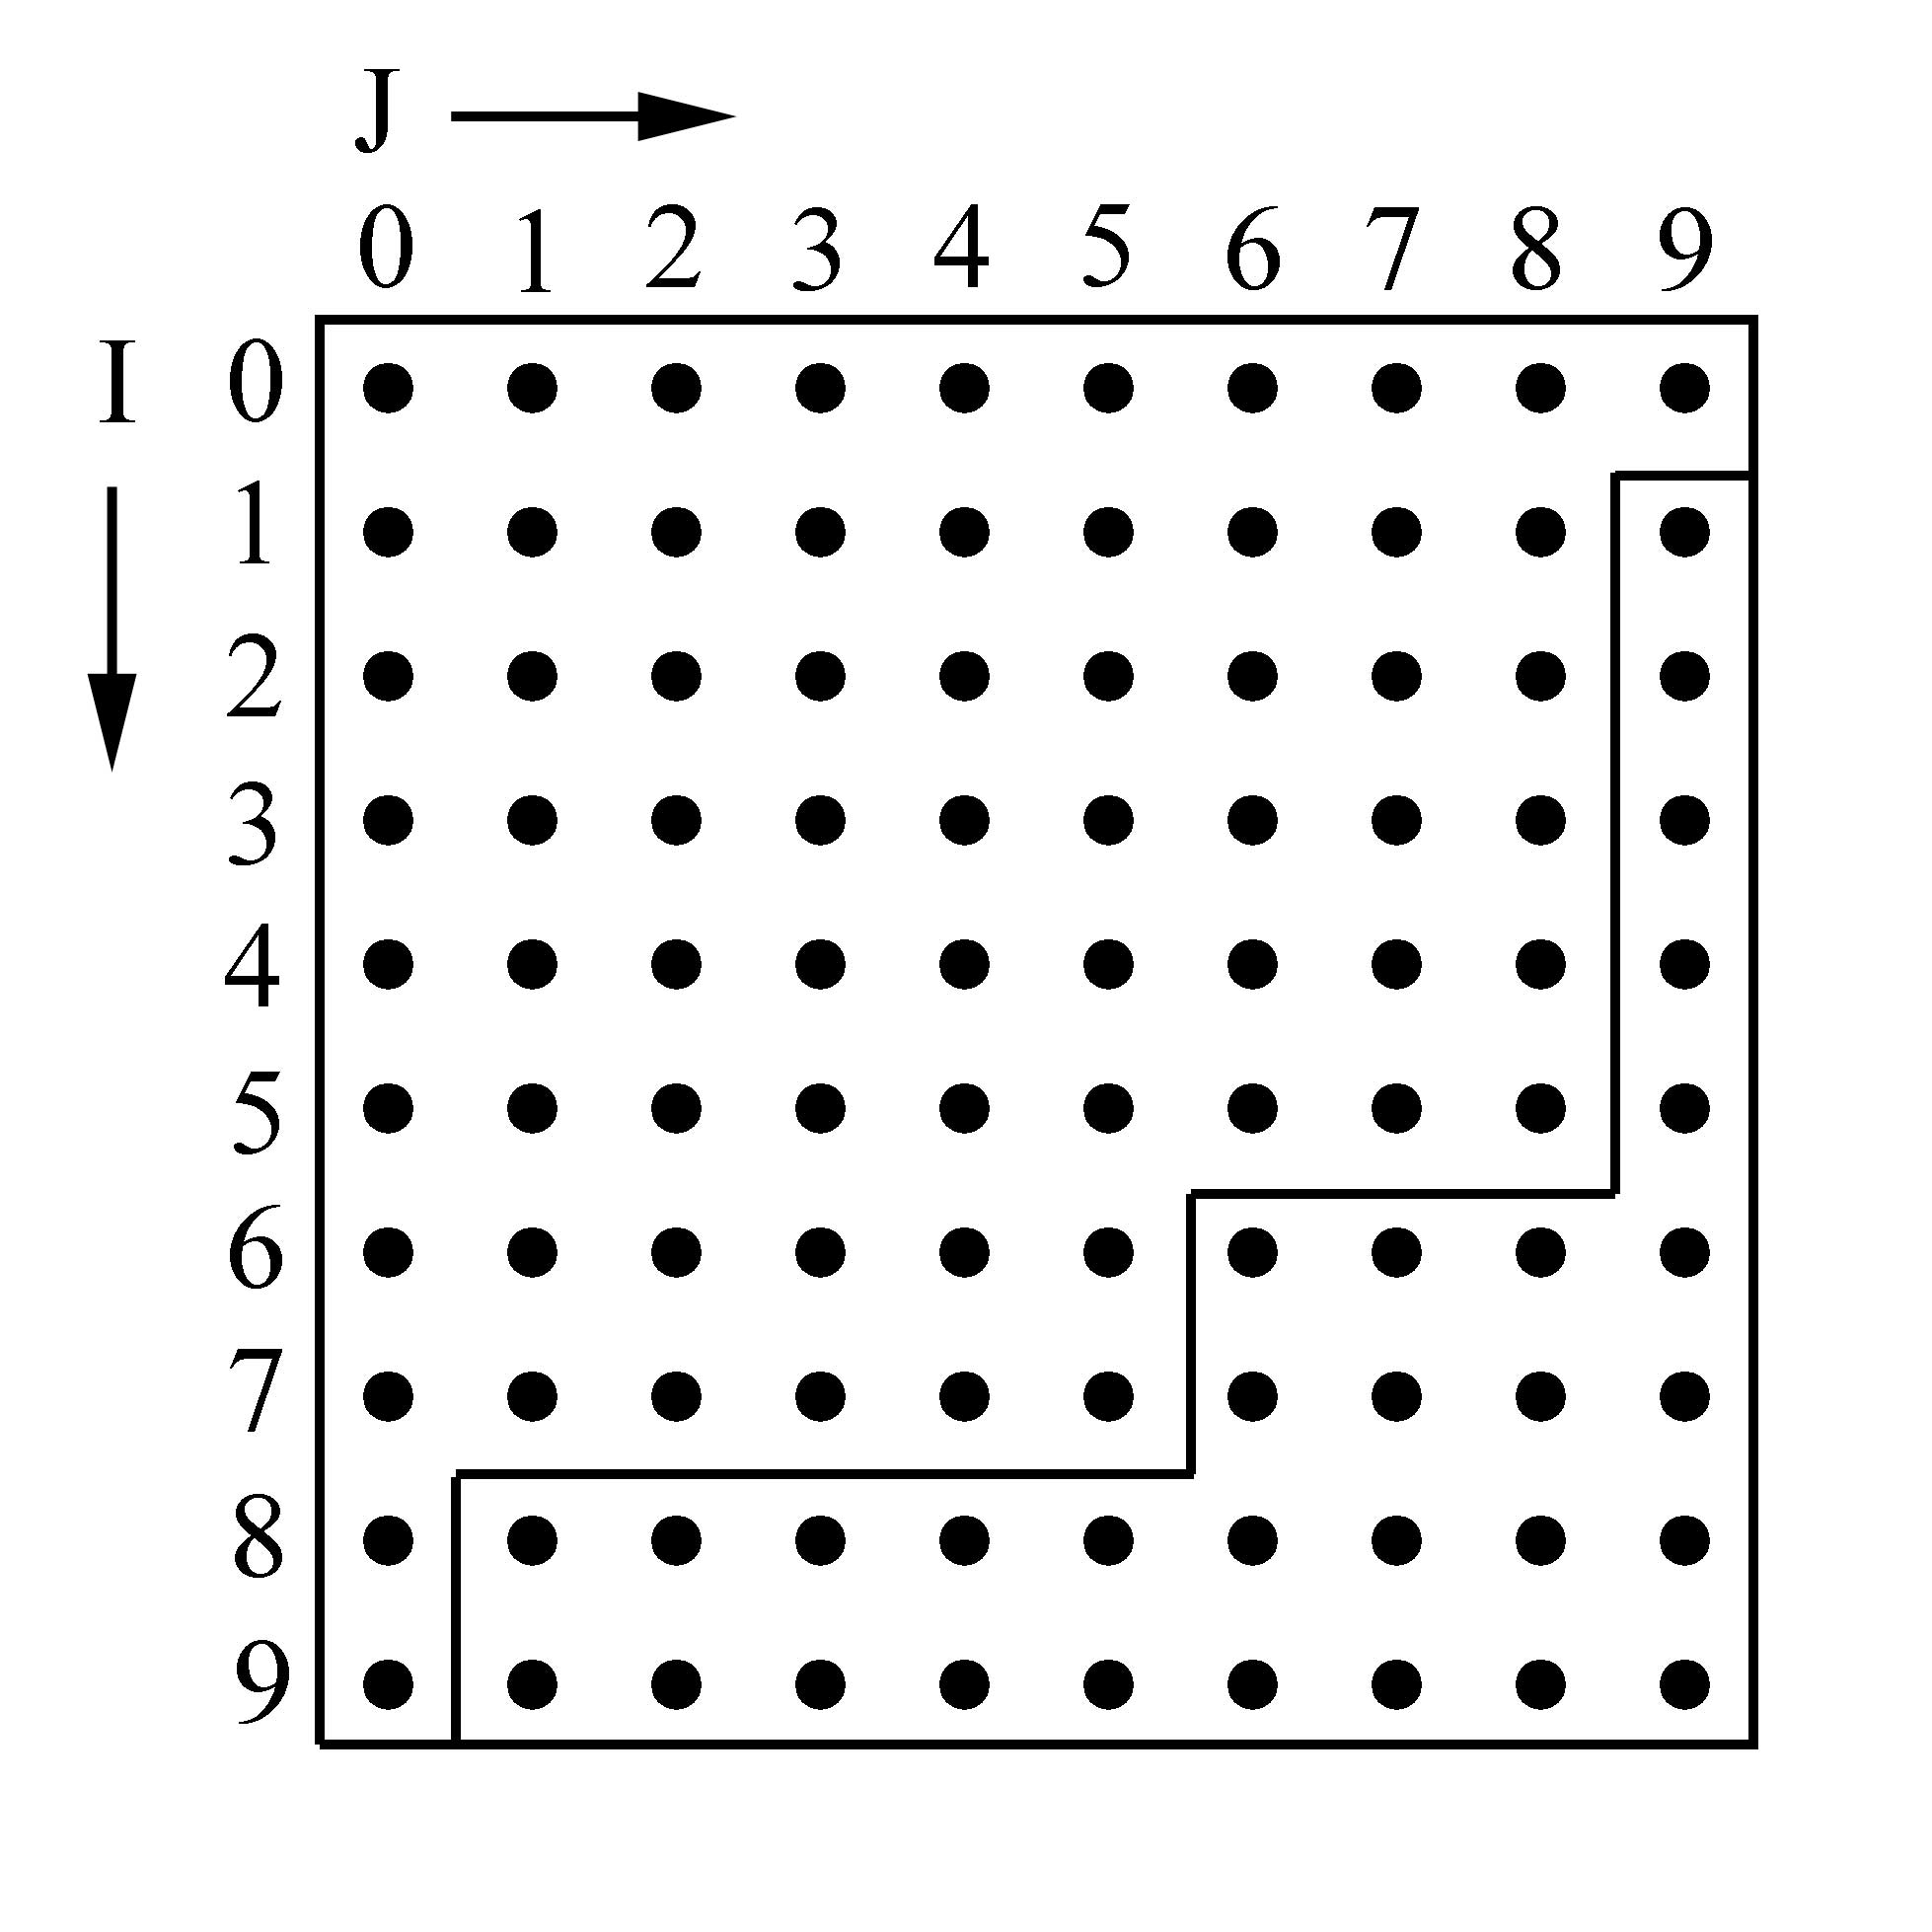
\includegraphics[width=\textwidth]{Figures/fig1b.jpg}
  \caption{}
  \label{fig:sub2}
\end{subfigure}
\caption{(a) Partitions by extended cycle shrinking algorithm. (b) Better partition}
\label{fig:eg_opt}
\end{figure}